\documentclass[border=3pt,tikz,12pt]{standalone}
\usepackage[utf8]{vietnam}
\usetikzlibrary{calc,angles,intersections,shapes.geometric,arrows,decorations.markings,arrows.meta,patterns.meta,patterns,quotes}
\usetikzlibrary{hobby}
\usepackage{tikz-3dplot,pgfplots}
\pgfplotsset{compat=1.15}
\usepgfplotslibrary{polar}
\usepackage{tkz-tab}
\usepackage{amsmath}
\begin{document}

	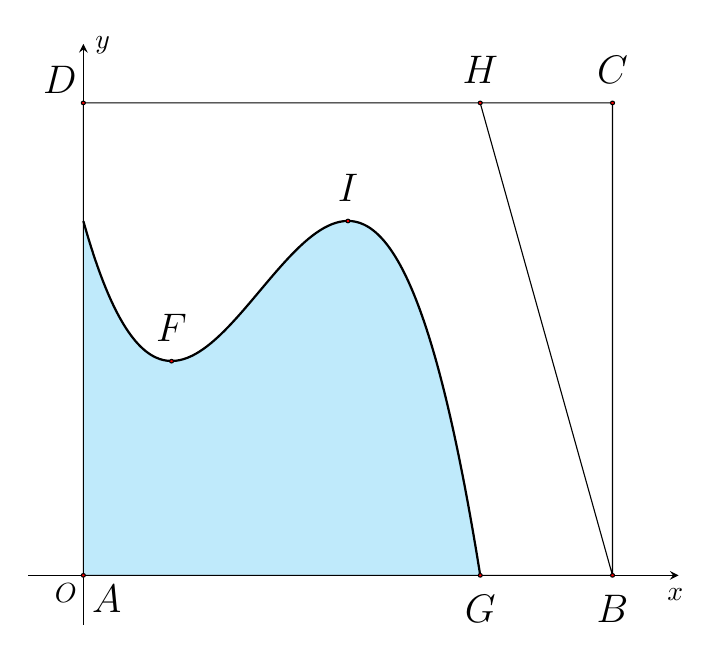
\begin{tikzpicture}[line cap=butt,line join=miter,>=stealth,xscale=0.56,yscale=0.5]
		\tikzset{declare function={xmin=-1;xmax=13;
			ymin=-1;ymax=13;
			a=-1/9; b=4/3; c=-4; d=9;
			xm=2; ym=5.44;
			xh=6; yh=9;
			f (\x)=a*(\x)^3+b*(\x)^2+c*(\x)+d;
			},
			smooth,samples=100
		}
		\draw[->] (xmin-0.25,0)--(xmax+0.5,0)
			node[shift={(-100:7pt)},font=\normalsize]{$ x $};
		\draw[->] (0,ymin-0.25)--(0,ymax+0.5)
			node[shift={(-5:7pt)},font=\normalsize]{$ y $};
		\fill (0,0) node[shift={(-135:9pt)},font=\normalsize]{$ O $};
%		\draw[dashed,cyan!75!blue] (xm,0) |- (0,ym) (xh,0) |- (0,yh);
%		\foreach \x in {-1, 1, 2, 3, 4, 5, 6, 7, 8,9}{
%			\draw (\x,2pt)--(\x,-2pt) +(0,-9pt) node[font=\scriptsize,fill=white,inner sep=1pt]{$\x$};
%		}
%		\foreach \y in {-1, 1, 2, 3, 4, 5, 6, 7, 8, 9}{
%			\draw (2pt,\y)--(-2pt,\y) +(-3pt,0) node[font=\scriptsize,anchor=east,fill=white,inner sep=1pt]{$\y$};
%		}
		\begin{scope}
			\clip (xmin,ymin) rectangle (xmax,ymax);
			\fill[cyan!25] (0,0)--plot[domain=0:9] (\x, {f (\x)})--(9,0)--cycle;
			\draw[thick] plot[domain=0:9] (\x, {f (\x)});
		\end{scope}
		\draw (12,0) coordinate (B)--(9,12) coordinate (H)  (12,0) --(12,12) coordinate (C)--(0,12) coordinate (D)--(0,0) coordinate (A)--cycle
		(9,0) coordinate (G)
		(6,9) coordinate (I)
		(2,ym) coordinate (F);
		

	\foreach \t/\g in {B/-90, H/90, C/90, D/135, A/-45,I/90,F/90,G/-90}{
		\draw[fill=red] (\t) circle (1.3pt) node[shift={(\g:12pt)},font=\Large]{$\t$};
	}
	\end{tikzpicture}

\end{document}
